\documentclass[11pt,a4paper]{article}
\usepackage[margin=22mm]{geometry}
\usepackage[T1]{fontenc}
\usepackage{lmodern,graphicx,booktabs,array,xcolor,hyperref,fancyhdr}
\definecolor{navy}{HTML}{173C5C}
\hypersetup{colorlinks=true,urlcolor=navy,linkcolor=navy}
\setlength{\parindent}{0pt}\setlength{\parskip}{6pt}
\pagestyle{fancy}\fancyhf{}\fancyhead[L]{\small Joana Owusu-Appiah | Research project report}
\fancyfoot[L]{\small Evidence checked: 15 September 2026}\fancyfoot[R]{\thepage}
\setlength{\headheight}{14pt}
\begin{document}

{\LARGE\bfseries\color{navy} CT Diffusion Counterfactuals}\par
{\large Guided image edits on an organ-recognition benchmark}\par
\textbf{Joana Owusu-Appiah}\par
Technical project report. This is not a peer-reviewed publication.

\section*{Research question and contribution}
Can classifier-guided diffusion reach an assigned organ class while keeping a CT-derived crop close to its input? This project trains a small organ classifier and an unconditional diffusion model, implements guided sampling, and measures the trade-off between target success and pixel change. It applies established diffusion methods; no new clinical intervention model is claimed.

\textbf{Summary.} The saved classifier reproduces 95.77\% test accuracy. In the original 256-image sampling sweep, 109 images reach the assigned target at noise level 200. A seeded repeat reaches 101 at level 200 and 102 at level 150. This supports an exploratory trade-off region, not an established optimum or anatomical-validity claim.

\section*{Real input data}
OrganAMNIST64, distributed by MedMNIST v2 and derived from LiTS, contains 11 organ classes. The supplied partition has 34,561 training, 6,491 validation and 17,778 test slices. Images are 64 $\times$ 64 uint8 crops, scaled to $[-1,1]$ for the models. They are preprocessed benchmark arrays, not raw DICOM or Hounsfield-unit images.

\begin{center}
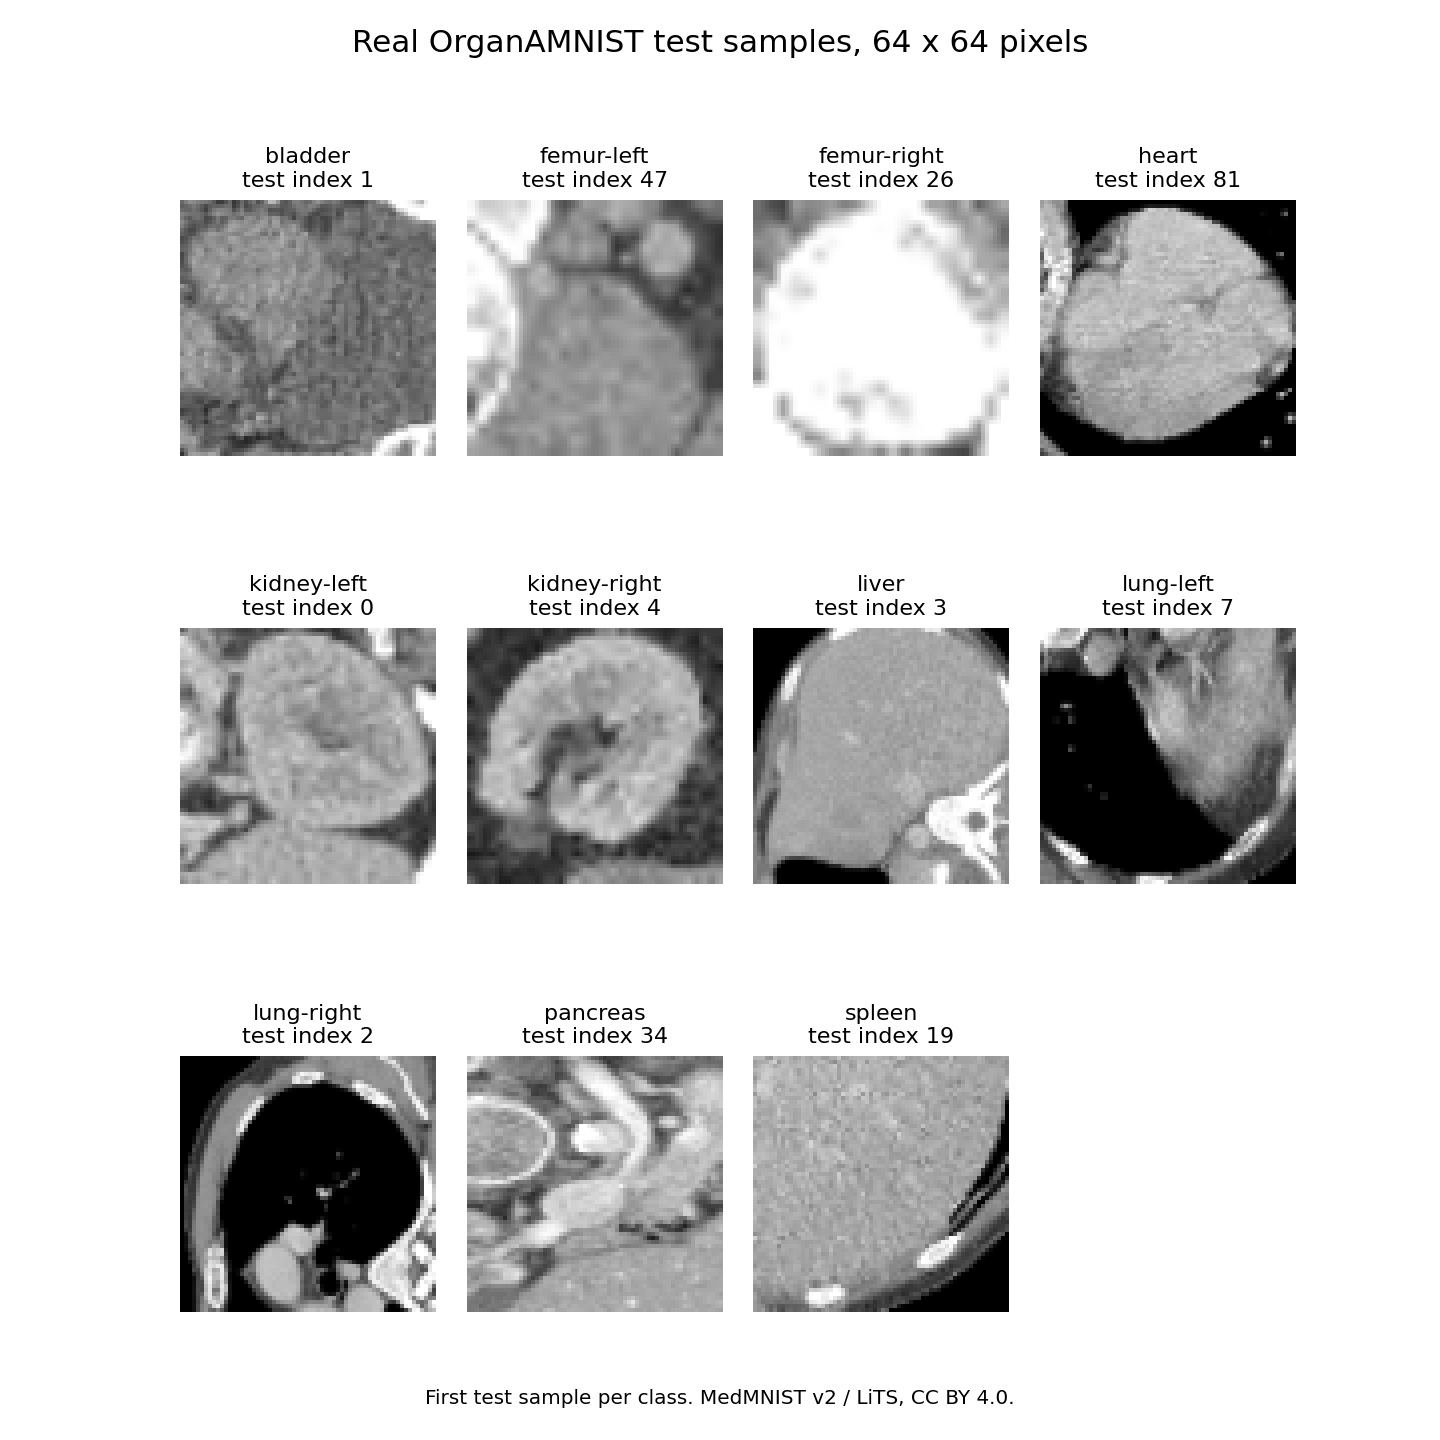
\includegraphics[width=0.66\linewidth]{../docs/figures/data_samples.png}
\end{center}
{\small Real test examples, one per class by first occurrence. Test indices appear in the panel. Source: MedMNIST v2 / LiTS, CC BY 4.0. Unmodified example arrays and hashes are included in the repository.}

\newpage
\section*{Method and evaluation}
The OrganCNN classifier is trained with cross-entropy for 15 epochs; validation accuracy selects the checkpoint. The MONAI diffusion U-Net is trained for 40 epochs to predict noise, with 1,000 timesteps, batch size 512 and learning rate 0.00025. Recorded training MSE decreases from 0.25735 to 0.03404; this is not held-out generative quality.

Sampling adds noise to a real input and denoises it with DDIM, using classifier gradients on the predicted clean image to guide toward a target organ. A 100-point DDIM grid is used, but only points at or below the starting noise level execute. Level 200 therefore uses 20 updates, not 100. Guidance scale is 6. The method does not guarantee a minimum-distance edit.

The sweep uses 256 test inputs selected with NumPy seed 0. Targets differ from the dataset label. Of these inputs, 239 are initially classified correctly; one is already predicted as its assigned target. Target attainment and actual prediction flips are therefore separate quantities.

\section*{Results}
\begin{center}\small
\begin{tabular}{rrrrr}\toprule
Noise & Updates & Original success & Repeat success & Original L1\\\midrule
50 & 6 & 22/256 & 23/256 & 0.0537\\
100 & 10 & 77/256 & 73/256 & 0.0904\\
150 & 15 & 99/256 & 102/256 & 0.1141\\
200 & 20 & 109/256 & 101/256 & 0.1551\\
300 & 30 & 96/256 & 98/256 & 0.3052\\
400 & 40 & 102/256 & 99/256 & 0.4217\\
600 & 60 & 56/256 & 56/256 & 0.4814\\\bottomrule
\end{tabular}\end{center}
The repeat uses PyTorch seed 2026 with the same checkpoints and inputs. At level 200 it records 100 actual target flips; 93 of the 239 originally correct inputs reach the target. These are repeated stochastic outputs on one subset, not independent validation cohorts.

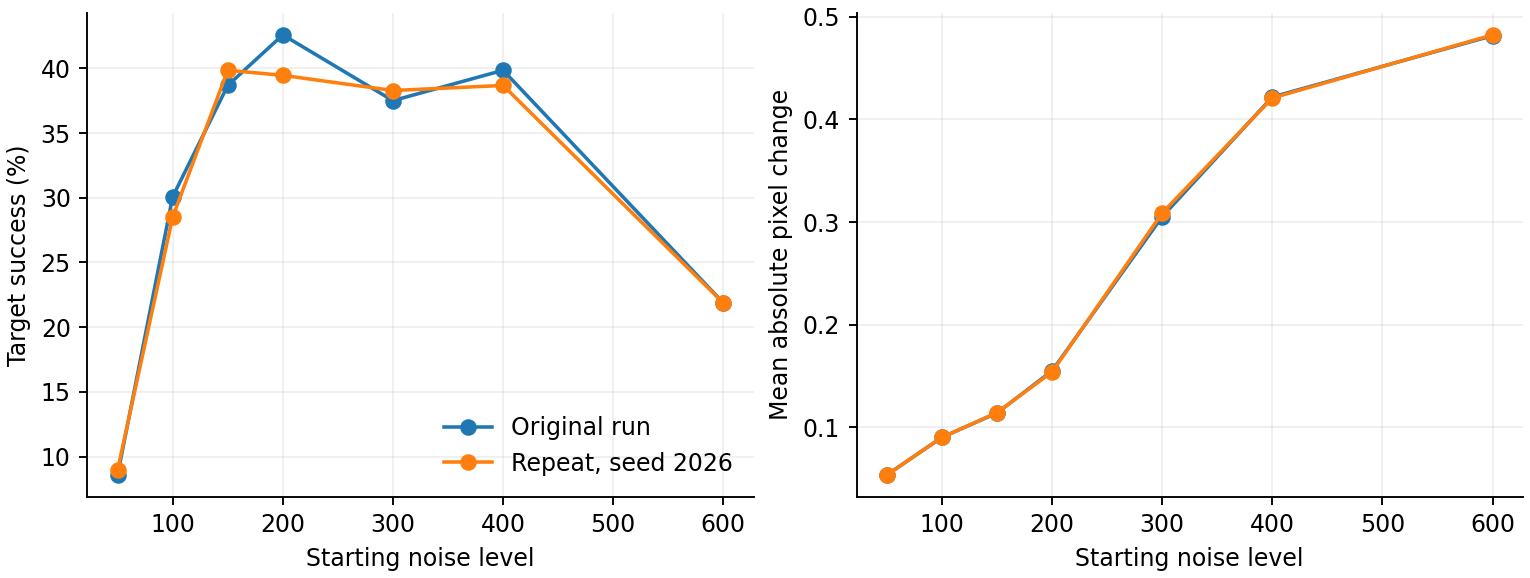
\includegraphics[width=\linewidth]{../docs/figures/replication.png}

At the original level 200, 54.6\% of pixels change by more than 0.1 in normalised units, with mean image correlation 0.866. Pixel proximity does not establish anatomical preservation. The best original noise level was selected using the test subset, so it remains exploratory.

\newpage
\section*{Sample quality and memorisation limits}
The original classifier-feature Fr\'echet distances, 46.84 for generated versus training images and 2.89 for real test versus training images, were reproduced. These are not standard ImageNet FID and do not validate clinical realism.

Although the saved tensor exposes 64 images, its backing storage retained all 1,024. All were recovered and published explicitly; the first 64 matched the visible tensor exactly. Recalculation reproduced the original sample-quality statistics.

Against 2,048 sampled training references, generated median pixel L2 distance was 22.68, versus 25.22 for 1,024 real test images. Generated images were closer by this measure. Against all 34,561 training references, the respective medians were 21.31 and 23.60. The minimum generated distance was 10.40, not zero.

This rules out exact pixel copies among these sampled outputs under this distance calculation. It does not exclude near-copying, memorisation in other outputs or patient-level leakage.

\section*{What was verified}
\begin{itemize}
\item Archive MD5, split counts, dimensions, intensity ranges and sample indices.
\item Full test-set classifier inference and all per-class accuracy values.
\item A new seven-level guided-sampling repeat, with indices and per-case predictions saved.
\item Original sample-quality statistics and pixel neighbours for all 1,024 recovered generated images against the full training pool.
\end{itemize}
Full training was not rerun. The original stochastic sampling state was not recorded. No radiologist review, segmentation-based anatomical check, disease intervention experiment or external clinical validation was performed. Patient and site identifiers are unavailable in the distributed arrays for an independent split audit.

\section*{Reproduction and evidence}
The repository includes small real-data examples, source code, original result JSON, per-case repeat arrays, a verification script and checked checkpoint downloads. Start with the CPU-only data preview, then follow the reproduction guide for inference and full checks. The audit used Python 3.11, PyTorch 2.14.0, MONAI 1.6.0 and an A100 80 GB GPU. Device changes can affect stochastic outputs.

\href{https://github.com/Joana-Mansa/ct-diffusion-counterfactuals}{Repository: Joana-Mansa/ct-diffusion-counterfactuals}\par
\href{https://github.com/Joana-Mansa/ct-diffusion-counterfactuals/blob/main/docs/verification.md}{Verification scope, raw evidence and checkpoint hashes}

\section*{Sources}
{\small
MedMNIST v2: Yang et al., Scientific Data 10, 41 (2023). \url{https://medmnist.com/}\par
MONAI implementation: \url{https://github.com/Project-MONAI/MONAI}\par
Jeanneret et al., diffusion-based counterfactuals: \url{https://arxiv.org/abs/2203.15636}\par
Atad et al., counterfactual diffusion autoencoders: \url{https://arxiv.org/abs/2408.01571}
}
\end{document}